%%%%%%%%%%%%%%%%%%%%%%%%%%%%%%%%%%%%%%%%%%%%%%%%%%%%%%%%%%%%%%%%%%%%%%%%%%%
%
% Generic template for TFC/TFM/TFG/Tesis
%
% $Id$
%
% By:
%  + Javier Mac�as-Guarasa.
%    Departamento de Electr�nica
%    Universidad de Alcal�
%  + Roberto Barra-Chicote.
%    Departamento de Ingenier�a Electr�nica
%    Universidad Polit�cnica de Madrid
%
% Based on original sources by Roberto Barra, Manuel Oca�a, Jes�s Nuevo,
% Pedro Revenga, Fernando Herr�nz and Noelia Hern�ndez. Thanks a lot to
% all of them, and to the many anonymous contributors found (thanks to
% google) that provided help in setting all this up.
%
% See also the additionalContributors.txt file to check the name of
% additional contributors to this work.
%
% If you think you can add pieces of relevant/useful examples,
% improvements, please contact us at (macias@depeca.uah.es)
%
% Copyleft 2013
%
%%%%%%%%%%%%%%%%%%%%%%%%%%%%%%%%%%%%%%%%%%%%%%%%%%%%%%%%%%%%%%%%%%%%%%%%%%%

\chapter{Implementaci�n software}
\label{cha_implementacion_sofware}

\begin{FraseCelebre}
  \begin{Frase}
TODO
La imaginaci�n es m�s importante que el conocimiento. El conocimiento es limitado y la imaginaci�n circunda el mundo.    
  \end{Frase}
  \begin{Fuente}
Albert Einstein, en \emph{The Saturday Evening Post}
  \end{Fuente}
\end{FraseCelebre}


\section{Arquitectura software}

\begin{figure}[H]
\centering
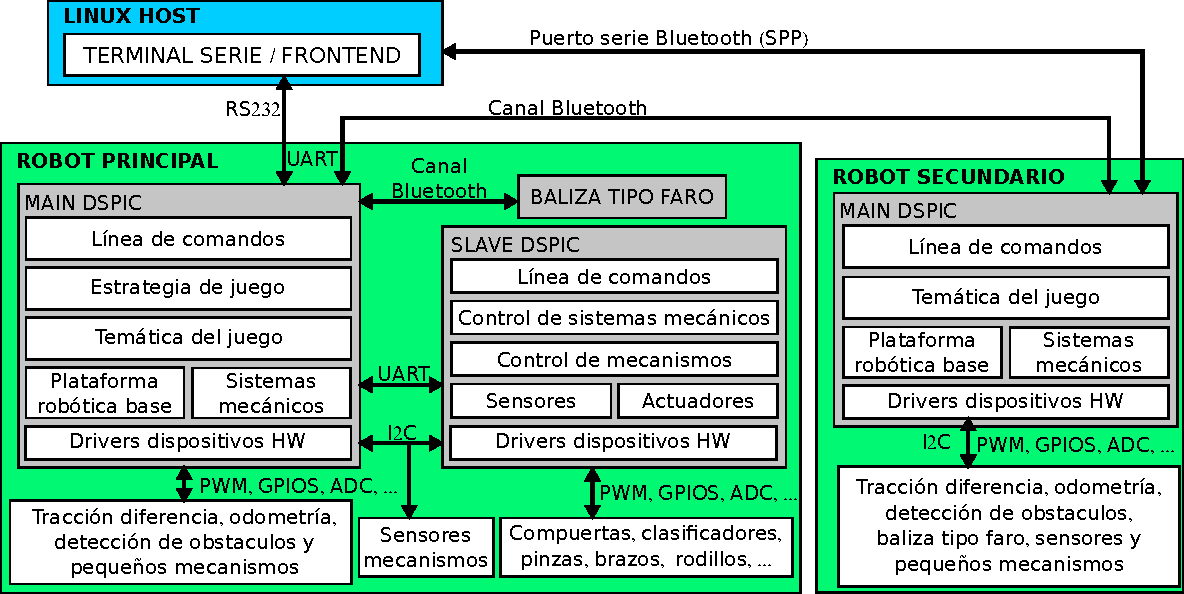
\includegraphics[width=\textwidth]{sw_diagrama_bloques}
\caption[]{Diagrama de bloques software del robot principal y secundario}
\end{figure}

\section{Drivers de dispositivos HW}

\section{Plataforma rob�tica base}

\begin{figure}[H]
\centering
\includegraphics[width=.9\textwidth]{Asserv_graph}
\caption[]{Diagrama de organizaci�n y funcionamiento SW de la plataforma rob�tica base}
\end{figure}

\subsection{Control de posici�n}
\subsection{Odometr�a}
\subsection{Detecci�n de bloqueos}
\subsection{Gesti�n de trayectorias}

\section{Abstracci�n robot}
[actuators | sensors | cs] > [strat (base, utils, avoid)] | [Interfaz baliza] | [Interfaz secondary robot]  

\section{Estrategia de juego}
[tareas secondary robot] | [tareas main robot] > [trayectorias a zonas | trabajo en zonas] > [estrategias partido]
%		\subsection{Estrategias de partido}
%			\subsubsection{Estrategia secuencial bloqueante}
%			\subsubsection{Estrategia reactiva}
%			\subsubsection{Estrat�gia basada en prioridades}
%			\subsubsection{Estrat�gia adaptativa}
%			\subsubsection{Estrategia con dos robots}

\section{Interfaz de comandos}

\section{Simulador de robots}

\begin{figure}[H]
\centering
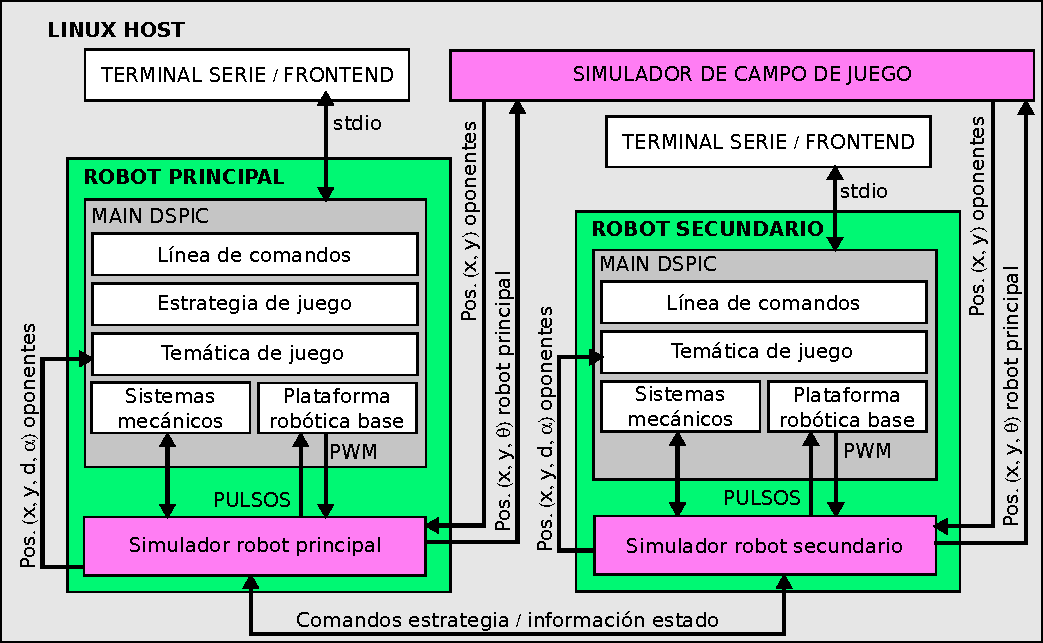
\includegraphics[width=\textwidth]{sw_diagrama_bloques_simulador}
\caption[]{Diagrama de bloques software del simulador de robots y campo de juego}
\end{figure}


%%% Local Variables:
%%% TeX-master: "../book"
%%% End:
